%% LyX 2.3.4.2 created this file.  For more info, see http://www.lyx.org/.
%% Do not edit unless you really know what you are doing.
\documentclass[10pt,english]{article}
\usepackage{mathptmx}
\usepackage[T1]{fontenc}
\usepackage[latin9]{inputenc}
\usepackage{geometry}
\geometry{verbose,tmargin=3cm,bmargin=3cm,lmargin=3cm,rmargin=3cm,headheight=3cm,headsep=3cm,columnsep=1.4cm}
\synctex=-1
\usepackage{mathrsfs}
\usepackage{amsmath}
\usepackage{amssymb}
\usepackage{graphicx}
\usepackage{setspace}
\PassOptionsToPackage{normalem}{ulem}
\usepackage{ulem}

\makeatletter
%%%%%%%%%%%%%%%%%%%%%%%%%%%%%% User specified LaTeX commands.
\usepackage{lscape}
\usepackage{longtable}
\usepackage{bbm}
\tolerance=1
\emergencystretch=\maxdimen
\hyphenpenalty=10000
\hbadness=10000

\makeatother

\usepackage{babel}
\begin{document}
\title{Status consumption and intertemporal substitution}
\maketitle
\begin{abstract}
\textit{A model for status consumption is derived based on the framework
for intertemporal consumption choice. Status is endogenised as states
of financial stability and included as part of the consumer's utility
in an intertemporal model for substitution between quality in non-durable
consumption and savings for future assets. Theoretical and numerical
solutions are discussed before estimation of the model for the Tanzanian
LSMS consumption microdata over the years 2010, 2012 and 2014.}
\end{abstract}

\section{Introduction}

In a conventional analysis of demand, the prices and quantities observed
for the items suggest the relative importance of commodities with
respect to each other. The demand for individual goods is often aggregated
into commodities to compare the demand with its past values or values
in a different population - thus providing a sense of quality for
a particular commodity. Evidently, a detailed set of market prices
of the goods within every commodity would be required if we were to
view status consumption as an instance of high-quality consumption
and use the measures of quality from the demand literature to measure
status-related consumption. As the data on market prices is seldom
available at local levels in most consumer surveys - we often use
a so-called hedonic approach - arguing that the characteristics of
the commodity are what consumers evaluate in forms of price. While
demand literature often uses market characteristics or shadow prices
for such analyses of quality for a particular commodity, the studies
on conspicuous consumption tend to explore a specific instance of
status consumption instead. Here, conspicuous consumption is expected
to occur through goods of a particular (visible) type that are meant
to be futile for the general needs of the consumer. This assumption
allows us to use to the separability of demand for visible goods.

In order to extend the concept of visible consumption in the developing
economies, we intend to use the framework of demand analysis without
this assumption of separability - arguing that the more general framework
could status consumption in a more varied context. While such a model
might not benefit from the tractability that the models for visible
consumption benefit from, the estimates of wealth of the consumer
(e.g. asset ownership in consumer data), if available, may allow us
to observe how quality across commodities is consumed with respect
to the wealth of the consumer. A general sense of status consumption
- as we argue - must come from a combination of higher quality across
commodities and a stable ownership of wealth or assets.

To elaborate the model, we enhance the framework for intertemporal
consumer choice by adding long-term incentives and near-term demand
for quality. In what could be seen as an attempt to refine a permanent
income approach (which vigorously ignores all non-monetary wealth),
we relate the consumption on quality with the long-term wealth proxied
with personal characteristics and asset ownership. Viewing owned assets
(durable items) owned as an indicator of wealth also comes in handy
as the data available on income is often poor in the economies with
a significant informal sector. In the environment of long-established
income and asset inequalities, the high quality commodities are seen
as the consumer's attempt to improve her perceived status. Arguing
that consumption is myopic and depends on the perception of status
in a near-term while savings are cumulative in an intertemporal model
for consumer choice, we let the representative consumer in the model
optimise a utility inclusive of status - which is obtained both by
owned assets (including skills and characteristics that are acquired
over multiple generations) and the quality of consumption. \uline{Since
the }signalling benefit a consumer derives from consumption, must
come out of either high-priced non-durable consumption or long-term
durable consumption, we view the signaling as the utility obtained
from the consumption of quality and owned assets over time.

The key variables that the econometric methods arising out of this
intertemporal substitution approach are concerned with are i) the
extent to which the consumers maintain their habits of purchasing
quality ii) the extent to which they choose to save for future assets
rather than to overspend on higher quality in the current time period
(measured simply as the distance - in monetary terms - from the cost
of basic needs) and lastly iii) a measure of the cost of basic needs.

A consideration of the cost of assets available to the consumer is
of particular interest if we wish to compare status-related consumption
in two economies with disparate levels of economic development (e.g.
a developed economy and a developing economy). The distribution of
assets - which may vary significantly in a developing economy from
the distribution in a developed economy - provide us a way to compare
the contexts of status consumption in the two economies. For a set
of assets (long-term durable goods) $\mathscr{D}$ ordered by increasing
cost, the difference in successive costs i.e. $\Delta d_{j}=d_{j}-d_{j-1}$
where $d_{j}\in\mathscr{D}$ and $d_{i}<d_{j}\forall(i<j)$ may be
much higher relative to the cost of quality consumption in one economy
relative to that in the other. These may have disparate effects on
consumer choice in the two economies as the costlier long-term assets
may discourage savings for the future (the consumer may give up hopes
of acquiring assets if she is to remain in a low income group relative
to asset costs) and the perceptions of high mobility may encourage
the consumer to overspend on quality in the short-term (matching one's
consumption to one's perceived status). As assets have a more definite
impact on the consumer's secure long-term growth (assets being a stronger
indicator the stability of her income), in equilibrium, the consumer
would balance the more uncertain perception of her status with the
more certain expected value of savings in her lifetime. Thus if income
is assumed to follow a process $i_{t}$ and the consumer spending
on her needs $\eta$ is known, then observing the proportion of consumer's
spending on quality (which also determines the savings rate for durable
goods in the intertemporal settings due to the total income constraint)
with respect to the measures of wealth can help us comment on the
contexts of status consumption in the two economies. This we believe
is key to understanding status consumption across economies.

The model we propose essentially compares the demand for long-term
items vs that for demands short-term quality. Including assets and
quality in a utility function, we consider the advantage from accumulated
assets as well as that from the quality in the near term. Observing
that a lot of non-durable consumption is related to the assets one
owns, we also introduce a cost associated with owning assets in the
intertemporal substitution framework. This explains how low income
could create a trap of low-asset ownership for the consumers. In summary,
we attempt to view status-related consumption in a conventional model
for consumer demand - using the availability of asset costs in an
economy and a definition of quality. We justify an interpretation
of status consumption from quality and assets based on the assertion
that for a rational consumer to spend on status consumption, she must
see some status utility from consumption in the long-term or the short-term.
To compare the status consumption in any two countries using our model,
we seek econometric methods that measure the supply issues in the
two economies and condition the demand on the macroeonomic differences
in the two economies. Quality of consumption is measured as the distance
of expensive nondurable consumption from the minimum cost of needs
and any status value to the consumer in the short-run is assumed to
be achieved through only the relative quality of consumption. The
two primary goals we that our approach wishes to accomplish is i)
to test whether the preference for quality increases with rise in
income and urbanisation (indicated by the expansion of consumer basket)
and ii) to see if preferences for quality change across populations
segregated through levels of development, economic strata or social
identities within an economy.

\section{Literature Review\label{sec:LiteratureReview}}

Status consumption was notably elaborated by Veblen \cite{VeblenLeisureClass}
in his 1899 treatise titled ``Theory of the Leisure Class''. Around
the time when Marx had endorsed a view of all commodities as products
of labour (diamond and corn alike), Veblen sought to explore the psychological
basis for consumption among the economic classes. At times, his view
of status consumption may appear critical of the ``bourgeois'' wastefulness
\footnote{``Throughout the entire evolution of conspicuous expenditure, whether
of goods or of services or human life, runs the obvious implication
that in order to effectually mend the consumer\textquoteright s good
fame it must be an expenditure of superfluities. In order to be reputable
it must be wasteful.''\cite{VeblenLeisureClass}} - but Veblen doesn't dwell upon the equivalence of labour for exchange
of commodities. While he observes the tendency amongst the elite to
distance themselves from physical labour - he argues that this tendency
has transformed itself into a desire of displaying exploits and has
survived in the culture from more primitive hunter-gatherer and agrarian
societies. This symbolism - he argued - is inherent in all exchange
of goods and services (including devotion and education \footnote{``The adoption of the cap and gown is one of the striking atavistic
features of modern college life, and at the same time it marks the
fact that these colleges have definitely become leisure-class establishments,
either in actual achievement or in aspiration.''\cite{VeblenLeisureClass}} ). 

The advancements of the last century in game theory and statistics
have made us revisit many of Veblen's observations in more precise
and quantitative terms - allowing us to interpret his early observations
on the seeming irrationality of consumer behaviour with a framework
for decision under risk. An understanding of the effect that human
behaviour and social conditions have on a macroscopic level may still
be far from complete\cite{StraussEcoGeo2008}, but the framework for
decision under risk is very pertinent to status-related consumption.
There are two threads in the literature that we find promising in
this regard. The first is that of habit formation amongst consumers
and the second on the relevance of social identities in visible consumption.
We believe that a framework of decision under risk should allow us
to link the two threads in the literature.

The literature from behavioural economics, marketing research and
development economics all seem to concur on the tendencies of habit
formation in consumer behaviour. The measurement of changes in habits
and quality has a long tradition in neoclassical economics (see Fisher-Shell\cite{FisherShell1968}
for a classical treatment of the problem). Of particular interest
is the model for myopia amongst consumers described by Muellbauer
\cite{MuellbauerRationalityMyopia1988.} who notes the significance
of lagged consumption on aggregate consumption. The life-cycle model
used by Muellbauer has been of considerable importance in more recent
studies on consumption where a rational utility-optimising consumer
balances between the non-durable and durable consumption based on
her planned savings over her life-time i.e. in an intertemporal substitution
setting (a problem often treated equivalent to the classical utility
maximising consumption problem). Improving upon the classical approach
where the consumer is subservient to her optimised plan for life-time
savings and consumption, a few behavioural approaches (see Shefrin-Thaler
\cite{ShefrinThaler1988} for example) have sought descriptive models
for mental accounting and factors such as willpower to better understand
the development of habits in consumers. Unlike in the classical variants
of the theory of consumer choice, the representative consumer in such
models is subject to overeating, overspending, accumulating items
she doesn't need or acquiring habits she cannot afford.

Another thread of literature on consumption that is more empirical
in nature has observed how social identities play a role in status-signalling.
Empirical studies in both the developed world and the developing countries
find social group identities relevant to status-related consumption
(see Chao et al. \cite{Chao1998}, Charles et al. \cite{CharlesHurstRace},
Omori et al. \cite{OmoriSmithVisRace}, Kaus\cite{KausSA}\textbf{
}and Khamis et al.\cite{ZahraIndia}). We belive that viewing status
consumption with the intertemporal substitution framework could help
connect the two threads in the literature.

A general approach that can help incorporate social order in consumption
has been presented by Corneo et al \cite{corneo_snobbism} and Coleman\cite{ColemanSocialTheory1990}
who motivate the case for a ranking order of status where a consumer
attempts to move herself up in the ranking order. With a framework
of social ranking and signaling therewith, Robert Frank\cite{FrankPond}
for example, finds that signaling needs become more important amongst
the lower economic strata when they are huddled in the overpopulated
suburban areas of big cities in the US. Inspecting similar behaviours
in South Africa (see Kaus\cite{KausSA}), Chai et al.\cite{ChaiKaus2019}
present evidence that the conspicuous consumption for consumers in
S Africa is relative to lower or similar income-groups (rather than
relative to higher income groups) . 

While the instances of status consumption under several cultural contexts
seem to have a common theme of expenditure on signaling items - there
may be a need to tread with caution when looking at demand of items
in the developing countries that are considered conspicuous in the
developed countries. This is because the relative wealth differences
may be more relevant for status differences in the developing countries.
The wealth differences being much larger and the industrial development
much more concentrated in a developing country, the glaringly visible
and sufficiently local (dense) wealth differences may have far more
weight than the limited range of status items that a rational consumer
may purchase (see Ustuner-Holt\cite{UstunerHolt2010} for criticism
of a \textit{belle epoque }view of status consumption). On the other
hand, rapid industrialisation and a transformation of consumer markets
in many developing countries in sub-Saharan Africa as well as Asia
may imply a narrowing the income differences in the consumption and
expansion of the industrial sector. These may make the consumption
of status-related items significant enough to make Veblen's ostensibly
dated insights on status relevant in the context of the developing
countries.

The sociological studies have long indicated the role that industrial
goods and income rises play in addressing of status needs by the consumers
(see Srinivas\cite{SrinivasSanskritization} , Ustuner-Holt\cite{UstunerHolt2010}
). In India of the 1950s, for example, Srinivas\cite{SrinivasSanskritization}
noted an instance of Veblen's pecuniary emulation\cite{VeblenLeisureClass}
(referred to as \textit{Sanskritization}) as the erstwhile lower classes
emulated the habits of higher social classes with their newly acquired
economic freedoms. In sub-Saharan Africa, the habits of the upper
economic classes were similarly observed to have expanded to the middle
and lower classes in the decades after the second world war. In the
post-feudal societies all over the world where consumer markets have
developed, a new working class seems to have replaced the feudal or
colonial order of the century before - attempting to emulate the former's
behaviour. Still, while this setting is not unrelated to the one that
Veblen had described in his treatise on conscpicuous consumption,
there are many ways in which the context of the sub-Saharan African
context is different from the American gilded age. One may find therefore
that the status consumption in the developing countries in large part
is merely an indication of wealth (see Khamis et al.\cite{ZahraIndia}
\footnote{The questions in the consumer survey (which is how a researcher may
obtain the list of visible items) may need to be adjusted to include
items that may indicate wealth. This is because the criteria of what
items are of visible importance is not enough for identifying status
consumption in an environment where wealth differences are both wide
and visible.}).

A model of the particular conditions of the post-war developments
that would consider the much higher levels of industrialisation and
population growth since the last century - is probably key to understanding
how the consumption is fundamentally different in our times. A model
reflecting such conditions that has been of significant interest in
the development economics literature is the Harris Todaro model\cite{GollinLRF,HarrisTodaro1970}
- which focuses on the urban and rural interactions in the developing
countries while relating income differences with the consumer's uncertainty.
The represenative consumer in the model (a worker/farmer) is meant
to maximise her income and reduce the risk associated with it as she
is faced with the choice of migration to the urban areas. To include
relative income and wealth concerns in order to incorporate status-related
consumption, one could enhance the model by refining the migration
incentives to include goals of consumption quality and peer effects.
A flight to urban areas - after all - may not be merely an escape
from despondent circumstances but also serve as an entry to the expanded
urban consumption basket and a (perceived) promise of social mobility
- incentives that are of importance in any group behaviour.

Peer effects for consumption have also been considered in the developing
economics literature. One example is the Indian food budget squeeze
(where per capita calorie intake seems to have declined as per capita
income has increased) - which Sen\cite{Sen2005Calories,DeatonDrezeIndiaFood}
attributes to the rise in the poverty-level for consumption of non-food
items. More recently, Chai et al \cite{ChaiKaus2019} have used a
peer-effects approach to inspect the consumption on signaling items.
In Sen view or in a general model considering long-term choices (e.g.
migration, ownership of a house etc.) with the relative consumption
of quality, a reference point separating basic needs from luxury or
high-quality consumption becomes a necessity. For much of the developing
economics literature, this encompasses the discussion of poverty levels.
In the developed economies where income inequalities are less of a
concern and data on income is generally more reliable, it is relatively
easier to separate the bare necessities from the luxuries to identify
status consumption. Focusing on ``visible'' consumption in the regions
of erstwhile East and West Germany after the economic liberalisation
at the end of cold war, for example, Friehe et al \cite{FrieheGermany}
have explored if prolonged measures of income equality can influence
conspicuous consumption asymmetrically when there is a sudden rise
in incomes. To develop a model with the effects of income and wealth
differences in a more general setting however (e.g. that of a developing
economy), one needs a clear definition of what constitutes the needs
of the consumer and her consumption for status. Without a clear separation
between needs and quality (or luxury) that is also general enough
to be used across cultural contexts, the macroeconomic factors, issues
of supply (e.g. income inequalities, distribution of resources etc.)
may appear so intertwined with the needs of the consumer that a robust
measure of status consumption can never be justified. 

In the literature we have surveyed, the methods to standardise the
macroeconomics inputs (welfare, growth, savings rate) and human needs
have appeared far more rigorous than a definition of status-related
consumption that is also general enough to be applied across various
cultural contexts. The conspicuous consumption studies appear to make
varied assumptions about what to include as part of conspicuous consumption
and what not to. Some studies, for example, include long-term durable
goods (e.g. housing) in the status-related items while others don't.
In some cases, studies employ a consumer basket identified from a
different economy on the basis of items being of conspicuous value
by common knowledge. Except when a survey is used to identify ``visible''
consumption, the contents of the consumer basket for conspicuous consumption
tend to have items that are just commonly understood to have some
signaling value (jewelry etc. that were first identified by Charles
et al. \cite{CharlesHurstRace}).

The visibility surveys (see Heffetz \cite{heffetz_visibility}) often
provide the means to get around the problem of the dependence of classification
of status items on a particular cultural context. The survey approach
to classification of status items also lends itself to tractable models
(e.g. those provided by Ireland \cite{ireland_signals}, Hopkins-Kornienko
\cite{HopkinsKornienkoStatusGames2004}). With an assumption that
conspicuous consumption brings no utility in the regular sense - an
argument often attributed to Veblen - the utility for visible consumption
may be considered separable (additively) from the utility for non-visible
consumption (we refer to this assumption as the futility assumption
henceworth) . This permits the empirical analyses to lump together
the demand for conspicuous items into one good. Despite this much
desirable tractability of visible consumption (see Ireland\cite{ireland_signals},
Hopkins-Kornienko \cite{HopkinsKornienkoStatusGames2004}), we favour
the an approach where snob and bandwagon behaviour form the fundamental
mechanisms for status consumption. The latter approach allows us to
include wealth differences and the quality in an intertemporal setting
- which we find more general for the varied contexts of the developing
world \footnote{The mutually opposing mechanisms that Veblen defined were pecuniary
emulation and invidious comparison - indicating the trends in consumption
where the not-so rich may emulate the rich (pecuniary emulation) or
show to the poor that they belong to a club that poor don't (invidious
comparison). We have found Corneo's terminology more tractable for
empirical analyses\cite{corneo_snobbism}.}.

A certain ontological sense of status can be associated with the consumer's
long-term security from the extreme fluctuations of in her wealth.
This ontological sense of status i.e. the consumer's long-term stability
of income is aligned with how status is measured in the literature
from health and sociological sciences - which often track status with
a vector of income, education and occupation (see Michelson et al.\cite{MichelsonMunizDeRose2013}
and Psake et al.\cite{PsakiSeidman2013} for a few examples). In the
short-term however, the multitude of risks perceived by the consumer
encompass the sense of status. This is the sense that is influenced
with short-term consumption. Treating assets accumulated as an indicator
of long-term wealth different from income, we use the intertemporal
substitution to understand how the consumers may balance consumption
in quality in the present with the savings for future assets. Thus,
in addition to the dispersion in income amongst social classes (gauged
with a simple variance in past income), we also consider the dispersion
in quality and wealth owing to long-established hierarchies. This
we believe is relevant to understanding the influence that wealth
yields towards status in the developing countries.

Empirically, the long-term assets which are considered part of the
consumer wealth are those that can be passed on to generations while
the short-term concerns of the consumer (which are themselves influenced
by the acquired wealth) comprise only of needs and quality. If there
is any status related utility to be derived from non-durable consumption,
it would be constituted in the felicity from quality (which is defined
as distance from needs). This is because the consumer with a habit
of high-quality in consumption (or deriving higher felicity above
the fulfillment of needs) would \textit{ceteris paribus }have higher
status than another consumer consuming less quality. The fulfilment
of consumer needs itself however carries no such influence on status.
Similarly, any status that is not signaled with non-durable consumption
i.e. quality must come out of long-term assets. 

Note that the utility to the consumer under the intertemporal setting
where she balances the two competing tendencies also considers the
peer effects which she faces. The utility function quantifies the
advantage a consumer receives by deviating from the the average values
of the particular status determinants (i.e. quality and asset ownership)
pertaining to the consumer's immediate surroundings (with respect
to a locality, a relevant social group, income or asset-owner group
etc.). \footnote{Quality differences may exist amongst the long-term assets as well.
However, if assets are sparingly available in the consumer population,
it may be suffice to consider the difference between having an asset
and not having the asset.}. If for example, the individuals with high asset ownership live in
a region different than where those with low asset ownership reside,
the consumer is not expected see so much benefit from consumption
of quality. The consumption of quality would thus be segregated based
on asset ownership or characteristics associated with long-term asset
ownership (e.g. region, social identity etc.). Since the social interaction
between groups segregated based on assets is minimised, this imposes
a constraint on the movement of consumption quality away from assets
(see the discussion of cost associated with asset ownership for a
further discussion on covement of quality and asset ownership).

\uline{While the models }for visible consumption can also be extended
to incorporate the peer effects, we find that an approach that endogenises
wealth and assets directly is more general for the developing world
context. So instead of using a framework for demand with a certain
items that are known a priori to have a status carrying potential,
we use a model which marks a substitution between the accumulation
of long-term assets or characteristics and the short-term relative
quality. By means of an analogy, consider a market for cars where
status is signalled through car ownership. The significance of visible
consumption means that the consumers pay more attention to outward
appearance of the car (the body work, paint, rims etc. - which definitely
futile) rather than the interior (engine cleaning, quality of tyres
etc.). But if we were to compare the signaling through car ownership
in the urban and rural areas, we would also want to see i) the price
differences in the cars being sold in the market and ii) the constraints
on occupation and income that exist in the respective areas. In the
context of status consumption, while it may be true that individuals
spend more on their outward appearances and visible goods (despite
controlling for everything else like occupation, income), visible
consumption is not all what status consumption over time may comprise
of (see the Figure \ref{fig:termsvenn} and Eastman \cite{Eastman1999}
for varied terminology around status consumption). Not all high quality
consumption is visible. In particular, some higher quality non-durable
consumption (such as using electricity in a developing country) may
not be visible in nature but must accompany higher durable consumption
that may in turn be visible (electrical equipment etc.). Similarly,
while a visible item is effectively a high-quality item (since visibility
is priced in the market), not all visible consumption may qualify
as high quality consumption either.

It is straightforward to include visible consumption in our framework
if it is viewed in relation to the ownership of assets or long-term
wealth. If the consumer preferences for needs across different commodity
groups and the assets she acquires are considered, visibility through
non-durable consumption (i.e. visible consumption) can be seeb as
a preference order for quality across the groups. More particularly,
as prices of commodities change or new goods are introduced, the consumer
may adjust her quality of non-durable consumption (once her needs
are met) based on a preference order over the commodity groups. For
example, a consumer may consider quality for transport more important
than quality in food (or vice versa). One could say that the commodities
such as food are less visible than household or entertainment.

In summary, the model we choose for long-term and short-term needs
does not view status consumption as futile but relates it with an
expectation of social mobility - which the consumer considers after
fulfilment of basic needs and which is influenced both with long-term
possessions and non-durable consumption. The relevance of a social-identity
to status is viewed in terms of an expectation of high status through
a history of past asset ownership, incomes/occupations (a criterion
that makes the consumer raise her expectations through association
with the identity). In the sections that follow, Section \ref{sec:Model}
details the model for intertemporal substitution we use to explain
status consumption. Section \ref{sec:Results} presents the results
we have obtained by using the model on the Tanzanian LSMS data.

\begin{singlespace}
\begin{figure}
\begin{centering}
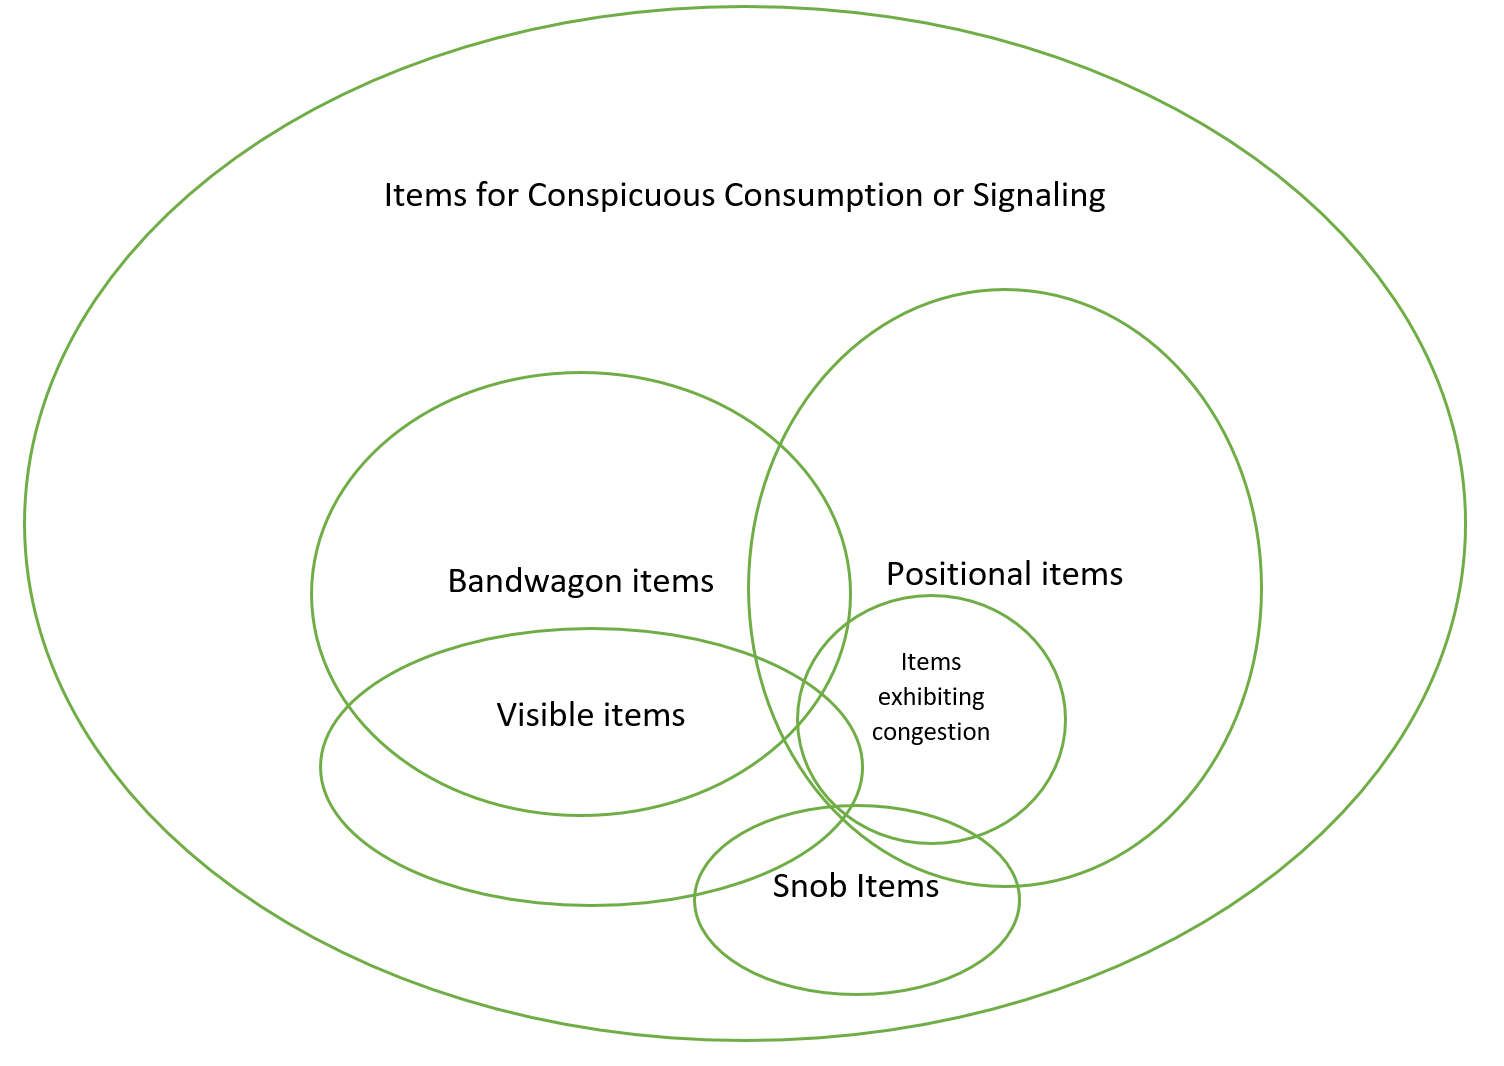
\includegraphics[scale=0.5]{conpicuous_cons_venn}
\par\end{centering}
\caption{\label{fig:termsvenn}A visualisation of various terms associated
with conspicuous consumption}
 
\end{figure}

\end{singlespace}

\section{Model\label{sec:Model}}

\subsection{Status as utility}

A property of utility function from where much of the model could
follow is that status is constituted in the consumer's long-term utility.
If not, the model's representative consumer would have no reason to
engage in status-related consumption in any form. As there is something
to be gained - however little - from non-durable status-consumption
(otherwise consumers would know of its futility), a consumer can a
achieve higher status in the model not only by the acquisition of
assets (which is assisted with higher income) but also by the status
promotion through consummption (which may enhanced social interactions
and improve self-image). The role of non-durable consumption is therefore
two-fold in the model - first, it addresses the immediate needs of
the consumer and second, it also matches the high-quality consumption
with status related goals. Quality or expensive non-durable consumption
provides both felicity in the present as well as a possible status
advantage - since all else being the same, someone consuming a higher
quality is likely to have more status than someone consuming a lower
quantity. \uline{Here}, we treat any expenditure above the basic
needs as an expenditure on quality or \textit{excess }- regardless
of what characteristics carrying quality are being priced in the market\cite{RosenImplicitHedonic1974,DeatonEconConsumer}
. We also argue that assets themselves would cause of this \textit{excess
}- thus segregating ways in which quality is consumed between those
who own assets and those who don't. A more detailed discussion of
such constraints follows in Section \ref{subsec:ModelDynamics}.

It is worth clarifying that by tracking the consumer's deviation from
her needs and matching consumption of quality with the consumer's
utility for status, we do not intend to make any descriptive claims
about the consumer's belief. Since consumption is myopic while savings
are cumulative, the association of a felicity from quality is only
a way to differentiate the more certain indicators of status from
those that contribute to the deviation from fulfillment of basic needs
in the short-term. 

It is also worth emphasising that conspicuous consumption should not
appear trivialised when viewed as mere higher-quality consumption.
We find that a lot of appeal for conspicuous consumption in the public
discourse is formed due to it being presented as a phenomenon that
only-serves-the-rich. Even though a conspicuous item is seen as an
item that is used both to distance oneself from the others and to
emulate the behaviour of those above oneself, there is a tendency
to focus more on its wastefulness amongst the rich than its utility
to the middle classes. A view that considers conspicuous consumption
a way to distinguish oneself from one's own reference group and the
reference wealth level through consumption would need to admit a more
general definition of status consumption that considers the effect
of the distance from fulfilment of basic needs on the the consumer's
signaling. If we can agree that the signaling behaviour can be exhibited
by everyone and cause a direct improvement of the consumer's perceived
status, then an increase in her consumption corresponding to her perceived
status is justified.

Another reason to object to the view of status consumption as a consumption
exclusive to the rich is that the utility to the rich from status
consumption might be quite little given that the rich consumer already
has enough to distance herself from others. Except for indicating
a membership to the club of its owners, the marginal utility a conspicuous
item offers to the rich consumer who may have just fallen short of
means to signal her wealth is much less than what it may offer to
the believers of social mobility who are trapped in an environment
of lower-asset ownership. The argument that considers conspicuous
consumption as only serving the rich may rule out conspicuous consumption
by the poorest who don't have anyone else to leave behind (much the
way the richest don't need to leave anyone behind). We argue instead
that even the poorest may want to indicate that they are not the poorest
- much the way the richest may want it to be known to the others that
they are indeed the richest\footnote{Any model of signalling or visible consumption\cite{ireland_signals,HopkinsKornienkoStatusGames2004}
can be used to make this argument.}. Made ubiquitous through expanding markets and increased awareness
of items through advertisement, therefore, signaling through non-durable
consumption is needed for everybody - as everyone in the middle (those
who are neither the richest nor the poorest) must also try to avoid
getting poorer and try to become the richest at all times.

A fundamental way in which our model differs from those of visible
consumption is that there is a private utility to be derived from
status consumption in the model. This warrants some clarification
as many empirical studies have viewed visible consumption as a kind
that provides only public utility (and no private utility). In the
view that motivates our model, a luxury watch may be futile for private
use by itself (when compared to its cheaper alternatives with same
functionality), but if an aspiring businessman uses his knowledge
of luxury watches to find new clients for her business, then the futile
consumption can translate into a material advantage. The perception
of status - however unrealistic - can influence one's wealth if everyone
in one's reference group also acts in accordance to the perception.
It may be apt to consider conspicuous consumption futile but only
in a sense that is different from what a modeler would be concerned
with. Items like luxury watches are important only because the rich
flock around them. Thus if the rich (the clients of our model businessman)
were to move away from luxury watches, the utility from the luxury
watches would be none. Admittedly, this is the sense in which conspicuous
consumption is always futile. However, the peer effects that conspicuous
items accompany is important as it acts as a means of connecting the
rich with the not-so rich. In the example of luxury watches, indeed
only a few of the purchasers of luxury watches would improve their
self-image - enhancing their social networks - while others may remain
mere purchasers. What matters is that a certain number of buyers of
luxury watches actually achieve success over the long term and influence
the peers in their reference group whose members can observe the success.
As explained before, we are not concerned with how many of the businessmen
actually believe that conspicuous consumption would help them (i.e.
we do not attempt to describe their beliefs).

In the operationalisation of the model, the long-term assets and the
income process provide the environment where the consumer's non-durable
consumption is observed. Here, the items or characteristics that are
passed on to the next generation are considered long-term assets while
those that cannot be passed are considered short-term. The factors
such as skills, education, class, identity etc. - which also contribute
the consumer's wealth and appear side-by-side with the long-term assets
in the model. 

\subsection{\label{subsec:UtilityOutline}Needs, wealth and consumption}

Having argued that both quality and ownership of long-term assets
contribute to the consumer's long-term status, we now turn to how
a consumer may achieve both in the context of needs and prices. Our
view of non-durable status-related consumption is essentially that
of non-necessary consumption - and thus empirically, it must rely
on a sound definition of needs - which provide the reference point
for quality in the model. That there must be the idea of universal
needs may itself be a contentious issue. On one hand, we have the
view that needs are determined solely by subjective preferences (see
Townsend\cite{DoyalGoughNeeds1991}) while on the other, there is
the view that a common man's needs can supersede her subjective interests
(wants). We lean towards an objective middle-path proposed by Doyal
and Gough\cite{DoyalGoughNeeds1991} who consider autonomy itself
- in addition to health - as a basic need of the consumer without
shunning the idea that the needs across cultural contexts should be
standardised.

In an empirical analysis, health and autonomy are fairly abstract
ideas when the context of consumption is not limited to food and employment.
When considering quality in food, for example, this is a relatively
easier task as we may just consider the cost of the cheapest option
for proteins, carbs, fruits etc. at the minimum subsistence level
in the local area. For contexts other than food, however, what constitutes
basic needs is less trivial. For example, what constitutes a basic
house or a basic set of furniture would require some justification
based on a cultural or geographic context. Standardising needs in
terms of the quantity of non-durable consumption poses another issue
- since the non-durable consumption may depend on the long-term assets
that the consumer possesses. In the household category for example,
a consumer with more electrical equipment would need more electricity
and thus a high non-durable consumption (while the consumer that does
not own any electrical assets would not have the respective non-durable
consumption). To get around the issue, we therefore consider needs
associated with a certain asset level. Once the level of needs in
a population of consumers is established, the cost of needs of the
consumer are driven the local price of the needs and a certain personal
characteristics (e.g. residence in an expensive region) as well as
the assets one possesses. This is discussed in more detail in Section
\ref{subsec:ModelDynamics}. 

It is worth highlighting that status is not considered a need using
this approach. Instead, it is inherent in the consumer's demand for
quality and the asset level she achieves while the her basic needs
are independent of her wealth. The aggregate sense of status through
consumption is derived by both assets and quality (across all commodities)
- driven by wealth and income of the consumer (rather than high-class
or low-class needs of the consumer). As an example, the difference
between the status of a rich and that of a poor family in our model
is not through disparate educational needs of the rich and poor children
but instead through a more general need for the family combined with
a demand for quality for education (with a higher price for higher
quality). It may thus be possible to proxy the needs of the family
simply by number of members in the family (adjusted by their age). 

The reference point of needs is crucial to our view of quality as
it is simply a measure of how far in price the consumption is from
the local cost of reference level needs. If the quality of consumption
or excess calculated in such a manner is $\nu$, the utility $\upsilon(\Psi,\nu,A)$
is a non-decreasing function of assets owned $A$, the cost of needs
$\Psi$ and $\nu$. Since consumption changes with the perceptions
of wealth, the dependence of $\nu$ on $A,\rho$ can give more structure
to the utility $\upsilon$. For example, while a consumer may want
to improve quality instead of saving for an asset, the quality $\nu$
may not be improved beyond a certain point until more assets are purchased.
For example, in the household category, high prices of housing may
encourage the consumer to upgrade accessories such as furniture (thus
improve $\nu$) but she may improve the quality instead of buying
a bigger house only until a certain point - beyond which she may need
a bigger house ($A$ ) to improve the furniture etc. (thus being encouraged
to save for $A$ again). Here, the consumption of quality $\nu$ moves
together with assets that the consumer acquires. In other words, there
are clusters of $\nu$ that are associated with a certain $\rho$. 

We discussion the modeling of peer effect in a later section but the
dependence of $A,\nu$ on $\rho$ also has implications on the additivity
of $\upsilon(\Psi,\nu,A)$. The limited substitution between assets
and non-durable consumption allows us to express the utility function
as $\upsilon=f(A)+g(\Psi)+m(\nu)$. As the consumer matches her consumption
with her status goals and a certain high quality non-durable consumption
is available only when associated with a corresponding asset or a
long-term characteristic (such as education, housing, identity, region
owing to segregation, trade barriers etc.), higher quality choices
would accompany higher-quality assets. The substitution between low-quality
asset and high-quality non-durable consumption being limited due to
co-movement of expensive non-durable consumption with expensive asset
ownership also means that the quality differences in the assets can
be ignored. A high-quality asset is thus merely a more expensive asset
in the utility $\upsilon(A,\rho,\nu)$ in the model.

We now consider how price derivatives may enter the utility and consumer
decision. Without price changes, the consumption of quality would
change only when individuals acquire long-term durable goods or give
up hopes of acquiring costlier assets (possibly due to other needs).
As the consumer would not sacrifice needs to purchase quality, a rise
in quality must come either from an increase in income or from an
undercut in savings. Similarly, if needs stay the same, a drop in
quality must be due to purchase of assets or a drop in income. Empirically,
the prices are attached with a commodity rather than overall quality.
So, to consider price changes, one must consider the price of needs
as well as the price of quality across the various commodities. Faced
with change in prices, a consumer may prefer quality in one commodity
over another (i.e. a consumer may switch consumption on quality from
transport to food or vice versa) as she addresses her needs and long-term
assets requirements. To illustrate this with an example, consider
a middle-income family that moves to a cheaper neighbourhood where
the rents are lower but the restaurants are fewer. The consumption
on fine-dining options - which signaled status and improved self-image
- can no longer take place. One way to view this change in the consumer's
circumstances is to observe that the price of entertainment services
are lower for the consumer in the new neighborhoods. Assuming the
needs of the family (indicated by the number of family members) haven't
changed, the consumption would either shift to saving for a better
car or improve quality in some other category (better jewelry, better
schooling for kids etc.) in response to price changes or a equivalent
changes in income. The sensitivity of consumption with respect to
price thus comprises of sensitivity with respect to basic needs $\frac{\partial c_{t}}{\partial\Psi_{t}}$as
well as a sensitivity with respect to quality for each commodity $\frac{\partial c_{t}}{\partial\nu_{t}}$.

\subsection{\label{subsec:ModelDynamics}Model Specification}

With the properties of the utility function discussed so far, we now
discuss how the observed variables which the consumer evaluates to
exercise her choice of quality that is turn measured as the distance
from cost of basic needs. These observed variables are the i) needs
of the consumer ii) her income and iii) the assets she owns. To measure
the quality chosen by the consumer, we observe the consumption within
certain categories (which for in the current chapter are food, energy,
transport and household). These variables are then assimilated in
the Euler equations of the intertemporal substitution problem.

The additive form of $\upsilon(\Psi,\nu,A)$ means that there is a
substitution between quality and assets. A consumer could achieve
the same utility - inclusive of status - as that of a consumer with
with higher education or higher asset ownership by raising her high-quality
consumption. Similarly, the asset-owners need not purchase quality
to stay ahead of others. Empirically, however, we note that high quality
in non-durable often is constrained by asset ownership. Those who
own a refrigerator spend less on kerosene for their energy needs compared
to those who don't own a refrigerator. If we measure quality as the
distance from cost of needs, there is a sunken cost the refrigerator
owner incurs due to her asset ownership. If we wish to view quality
after having conditioned for such costs in order to avoid double-counting
the advantage the asset owner has, we ought to separate the quality
demanded by the consumer from that which is incurred due to asset
ownership. To ask whether the refrigerator owners spend more on exotic
fruits than those those who don't, we must separate the running costs
of the refrigerator from the measurement of quality control $\nu$.
Two measures address this standardisation of demand - first is the
classification of quality in separable commodities e.g. food, energy
so that we may compare demand for quality in food with that for quality
in household goods or transport. The second is the introduction of
a cost-function $p(A_{t},\rho)$ - which accounts for the cost of
maintaining assets or similar characteristics (such as education or
social class) \footnote{It is possible that ownership of some assets generates some rental
income. Although we haven't found the significance of such income
in the consumption data, we would prefer to treat such income as an
additional stream of income instead treating it as negative costs
in the model.}. This takes care of the peer-effects to some extent - giving more
weight to quality consumed by non-asset owners than would be if we
didn't include the cost of assets.

\subsubsection{\label{subsec:NeedsProcess}Needs of the consumer}

As we have briefly discussed in the Section \ref{subsec:nonstochproblem},
our notion of quality is dependent on what we consider as needs rather
than the characteristics of items (see Rosen\cite{RosenImplicitHedonic1974}
for a summary of hedonic approaches). We define needs as the standard
requirements not meeting which would lead to a definite harm (this
is in accordance to the theory argued for by Doyal and Gough \cite{DoyalGoughNeeds1991}).
To an argument that a family can survive on just starch, the counter-argument
would be that a foreseeable damage to the health of the consumer incurred
by not having other nutrients is definite - thus ruling out a starch
diet fulfilling the set of dietary needs. However, such a theory of
needs is a normative concern (rather than descriptive) - as a consumer
may not always want her needs. Such a model for needs cannot represent
a situation where consumers forgo a certain need to compromise on
their health or autonomy in favour of some other wants. This makes
the task to ensure that the needs are indeed just a minimum necessary
set for health and autonomy to the individual extremely important.

We consider the minimum requirements for commodities such as food,
clothing, housing and employment and calculate the costs associated
with them in the local context (at a district level in the Tanzanian
data - for example). The needs are then adjusted based on the assets
one possesses. If a household possesses a car, then the needs of the
household are incremented with the petrol consumption per year. Thus,
some cost of needs (e.g. for food) are multiplied by the number of
household members in the family while other needs are calculated per
household to obtain the net cost of needs $\Psi$ for a household.
The details of the this process are explained in Section \ref{subsec:Needs-Cost}. 

Relying only on total costs associated with a commodity (i.e. without
using the quantity consumed), this notion of quality or \textit{excess
}cannot differentiate between the consumption of a higher quantity
and of a higher quality. Consider for example, a household with a
single member having consuming the quantity $q_{1}$ for a commodity
priced $p_{1}$. If the minimum requirement for basic needs is $\Psi=p_{1}q_{0}$,
then our quality metric for the consumer is $\frac{p_{1}q_{1}}{p_{1}q_{0}}=\frac{q_{1}}{q_{0}}$.
For the individual's household, consuming more quantity than the minimum
may increase the measure of quality much the way it would if she had
switched to a better quality. As the consumption surveys often don't
record the quantity consumed for non-food commodities e.g. clothing,
toiletries etc. (nor the associated brand information), there is no
way for us to distinguish between over-consumption and high-quality
consumption by relying solely on the total consumption on the good
(i.e. $p\cdot q=\sum_{i}p_{i}q_{i}=x$). However, as we do know whether
the range of goods within a commodity are available in the region
or not, it is possible to draw conclusions about over-consumption
and higher-quality consumption for a group of consumers - separated
by region or other characteristics - who face different ranges of
goods available within a commodity. This is particularly so when using
pseudo-panel analyses for the data.

\subsubsection{Income Process}

The goal of using an income process in the model is to provide an
exogenous way to differentiate increase in household incomes from
the accumulation of assets. It is the substitution of the latter with
consumption that is crucial to our interpretation of status consumption
as a scale of quality \textit{excess}.

Unlike in PIH, the accumulation of long-term assets have an influence
on the substitution between savings and quality in an \textbf{\uline{intertemporal
setting}}. What this means empirically is that while the exogenous
income process may depend on education or occupation levels, the effect
that long-term characteristics have on consumption are not necessarily
through income but through constraints that the long-term characteristics
bring. As the effects of on consumption are modeled explicitly, it
would suffice if the income process models an the monetary growth
i.e. a reflection of the steady growth in the economy on to the consumer's
budget. For the analysis of the Tanzanian data therefore, we have
assumed an income process dependent on long-term characteristics characteristics
such as education and occupation. 

\subsubsection{Change in asset ownership over time}

The wealth of a consumer is represented in the model with a combination
of accumulated assets and long-term characteristics (education, occupation
or social identity). The asset ownership is modeled with an asset
account - whose value is reflected in the total cost of assets inclusive
of cash assets that the consumer owns. The use of such an asset account
implies that no distinction is made between the accumulation of cash
reserved to purchase assets and the actual purchase of assets. Thus
if a consumer sets her eyes on assets $A$ and $B$ (that have prices
$\Pi_{A}<\Pi_{B}$) and the value of her cash account at time $t$
is $A_{t}=\Pi_{A}$, then the model does not distinguish between the
case when she buys the asset $A$ (price $\Pi_{A}$) and the case
when she forgoes the purchase of $A$ to save for the future purchase
of $B$ ( prices $\Pi_{B}>\Pi_{A}$). 

Another way to view the asset account is to consider that all assets
in the economy are managed by a large firm (owing its success to preferences
being the same for everybody) that provides furniture, housing and
all amenities at a flat upfront cost. Every asset and service - offered
as a life-long subscription - can be purchased by giving an amount
to this company. We also assume that at the of the lifetime of a consumer,
her personal wealth would either be consumed or would be passed on
to her progeny so that the asset account at the end of the lifetime
becomes starting wealth of some other household(s) in the economy.
Consequently, while all individuals in the population are assumed
to be the same as our representative consumer in terms of the preferences
for needs over quality, they differ in the the starting amount of
their asset accounts as well as the trends of their salaries, the
trajectory of their needs and their quality habits of quality (\textit{excess}).
If a consumer has a starting income $i_{0}$ and her salary after
$\tau$ years of working is $i_{\tau}$ then at a given time $\tau$,
she could have purchased assets from a portion of her income and decided
that she does not want more assets for the rest of her life. Alternatively,
her life circumstances might have changed (she may need a bigger house
or want a more expensive house) thus needing more assets urgently.
The consumption in the period $\tau$ would therefore depend on the
needs $\Psi_{t}$, asset account value $A_{t}$ and the consumption
of quality $\nu_{\tau}$ in the period $\tau$. Due to the minimal
presence of credit facilities in the developing countries, we assume
a negligible credit in the market. This in turn implies that the consumer
can only save to buy more of the only asset available in the market.

\subsubsection{\label{subsec:nonstochproblem}Dynamic Optimisation}

Given the variables - cost of needs $\Psi_{t}$, owned assets $A_{t}$,
income $i_{t}$ and observed consumption on quality $\nu_{t}$ that
are observed in the data, we now turn to a quality control in the
Euler equations of the intertemporal setting that represents the consumer
choice for quality. By definition of the needs, a consumer is meant
to select a quality control $\nu_{t}$ only after her needs and those
imposed by the owned assets $A_{t}$ as well as her personal characteristics
$\rho$ are fulfilled (the lack of subscript in $\rho$ is due to
the assumption that the personal characteristics don't change in our
near-term analysis). Thus we view the control for quality (\textit{excess})
$\nu_{t}$ (in period $t$) simply the distance in terms of money
from the cost of needs for the household. The higher its value the
higher would be the distance from the basic needs consumption (and
lower would be the future growth of $A_{t}$). Other than the control
$\nu$, the consumption depends both on needs and the long-term choices
of the consumer (which are encapsulated by the asset $A_{t}$ the
consumer has accumulated in the past and the the personal characteristics
$\rho$ she possesses).

The non-durable costs imposed by the assets one possesses (e.g. fuel
for cars, electricity for heating equipment, rent/maintenance-fees
for housing etc.) imply either that avoiding the respective expenses
is not an option for the consumer owning some assets or that some
certain long-term choices or characteristics (e.g. not having a house
or living in a region that doesn't have electricity available) would
limit the choice to avail quality through non-durable consumption.
For example, a homeowner is required to maintain her own house the
way someone who doesn't own the house has to pay the rent. As some
costs are incurred due to the assets that the consumer acquires, a
distance from the basic needs (which are themselves imposed only by
health and autonomy requirements) could be introduced as the consumer
acquires more assets. Such ``extended'' needs of the consumer as
she acquires assets necessitate a parameter in the model that is different
from the quality control $\nu_{t}$ and separates how much the consumer
choice is related to her long-term standing influenced by $A_{t}$
and $\rho$ from how much quality is demanded in the period $t$.
As discussed in the Section\ref{subsec:NeedsProcess} , we view these
constraints i.e. costs incurred due to asset ownership (e.g. of maintenance
fees or rent in the housing example) as part of the needs $\Psi_{t}$.
The effect of supply-related asymmetries in the data e.g. lack of
availability of certain goods in a certain region etc. are accommodated
in the costs $\Psi_{t}$. 

The simplest instance of intertemporal substitution is a two period
model where assets are meant to be liquidated at the end of the second
period. If one may assume that the relative preference of quality
over assets does not change over time, the utility to be optimised
by the consumer in the two-period model can be written as 

\begin{alignat*}{1}
U & =\beta_{1}(a\ log(\nu_{1})+b\ log(A_{1}))+\beta_{2}(a\ log(\nu_{2})+b\ log(A_{2}))
\end{alignat*}
 

Here, $\nu_{1},\nu_{2}$ are consumption on quality in periods 1 and
2 while $A_{1},A_{2}$ are that on assets in the respective periods
(assuming that needs do not carry utility )\footnote{An alternate equivalent form may be more intuitive $U=a(\beta_{1}log(\nu_{1})+\beta_{2}log(\nu_{2}))+b(\beta_{1}log(A_{1})+\beta_{2}log(A_{2}))$}.
In the typical solution of the intertemporal problem, the wealth constraint
could be written as $W=\frac{A_{2}}{(1+r)^{2}}+\frac{c_{1}-p_{1}}{1+r}+\frac{c_{2}-p_{2}}{(1+r)^{2}}$
so that Lagrangian $L=U-\lambda(W-\frac{A_{2}}{(1+r)^{2}}-\frac{c_{1}-p_{1}}{1+r}-\frac{c_{2}-p_{2}}{(1+r)^{2}})$
leads to the first order conditions $\frac{\partial L}{\partial\nu_{1}}=\frac{\partial L}{\partial\nu_{2}}=\frac{\partial L}{\partial\lambda}=0$.
Notice however that one cannot guarantee $\frac{\partial f(\nu_{2})}{\partial\nu_{1}}=0$
in the for the optimisation of $U$. This is where the boundary condition
of the final asset state being 0 (i.e. all of the consumer's assets
being liquidated and consumed in the last period) and a discount factor
for expected state (whose Euler equations are specified) help simplify
the optimisation problem\footnote{This solution a the non-stochastic intertemporal problem essentially
draws an equivalence between total wealth constraint $W$ and the
total outlay $x=\textbf{p}\cdot\textbf{q}$ of the classical consumer
choice problem ) before employing similar econometric methods. Recall
that $w=\beta ln(x)+\gamma ln(p)+\epsilon$ commonly used in estimation
is effectively derived from $w_{i}=p_{i}q_{i}/x\Rightarrow log(w_{i})=log(p_{i})+log(g(x,p))-log(x)$.
With $g(x,p)$ as the Marshallian demand function, using the double-logarithmic
model (which is a mere restatement of existence of elasticities through
total differentiation) yields $log(g(x,p))=\alpha_{i}+\frac{\partial log(g(x,p))}{\partial log(x)}log(x)+\frac{\partial log(g(x,p))}{\partial log(p)}log(p)$
and thus $log(w_{i})=\alpha_{i}+(\frac{\partial log(g(x,p))}{\partial log(x)}-1)log(x)+(\frac{\partial log(g(x,p))}{\partial log(p_{i})}+1)log(p_{i})+\sum_{j\ne i}\frac{\partial log(g(x,p))}{\partial log(p_{j})}log(p_{j})$. 

As the adding up restriction is more difficult to impose on this form
rather than the slightly modified : $w_{i}=\alpha_{i}+\beta_{i}log(x)+\gamma_{i}log(p_{i})$
\cite{DeatonEconConsumer}, the latter is the more popular choice.
An estimation of demand elasticities of consumption can be performed
with parallel arguments using the total wealth constraint $W$. In
this equivalent formulation, the constraint for the consumer can be
stated as the total wealth $W=\delta_{i}(A_{T}+\sum c_{i})$ where
$A_{T}$ are the assets accumulated over the period $T$, $c_{i}$
the consumption in period $i$ and the discount factors can be chosen
as$\delta_{i}=\frac{1}{(1+r)^{i}}$ (this holds even if one assumes
that $A_{T}$ is 0 at the end by the consumer spending everything
as $c_{T}$ at the end of period $T$). Equivalent to the case of
income constraint $\textbf{p}\cdot\textbf{q}=x$ for the maximisation
of $\upsilon(\textbf{q})$, the wealth constraint $W$ is meant to
be known to the representative consumer i.e. the consumer chooses
a plan for $c_{i},A_{i}$ knowing what her total wealth $W$ and future
expectations of prices are.}. Since we consider the final state of assets exogenous in our model,
we take a slightly different approach with the formulation of a dynamic
optimisation problem.

If the initial and final asset levels known, the Euler equations can
be written as follows:

\begin{alignat*}{1}
A_{t+1} & =A_{t}(1+r)+i_{t+1}-\nu_{t+1}-\Psi_{t+1}
\end{alignat*}

Above signifies that the consumer may consume quality $\nu_{1}$ and
$\nu_{2}$ ( $\nu_{0}$ and $\nu_{3...}$ being undefined) in the
periods 1 and 2 while she bears the cost of the needs $\Psi_{1},\Psi_{2}$
(in periods 1 and 2 respectively). The intertemporal substitution
setting means that she may save for asset growth to $A_{1}$ and $A_{2}$
instead of consuming all her income $i_{t}$ as $c_{t}=\nu_{t}+\Psi_{t}$
i.e. she can spend all her income $i_{1},i_{2}$ as $c_{1},c_{2}$
(respectively) or save some of it towards $A_{1},A_{2}$. If initial
conditions are $A_{0}$ (the starting wealth), the rate of growth
of money (interest rate) and an exogenous income process $i_{t}$
are known, we can expand the the Euler equations as follows:

\begin{gather*}
A_{1}=A_{0}(1+r)+i_{1}-c_{1}=A_{0}(1+r)+i_{1}-\Psi_{1}-\nu_{1}\\
(\because c_{1}=\Psi_{1}+\nu_{1})
\end{gather*}
 

Similarly, 

\begin{alignat*}{1}
A_{2} & =A_{1}(1+r)+i_{2}-\Psi_{2}-\nu_{2}
\end{alignat*}
 Assuming that we observe both states of the wealth, $A_{0},A_{1}$
and $A_{2}$, as well as $c_{1},c_{2},$$\Psi_{1},\Psi_{2}$ we can
then to solve for the parameters that govern the utility function
additive over time $u=u_{1}+u_{2}$ . 

Here, $u_{1},u_{2}$ are utilities over periods and 1 and 2 (respectively).
To motivate the dynamic optimisation approach, consider the consumer's
choices in a one-period consumption - where she could either spend
all income $i_{1}$ as $c_{_{1}}=\nu_{1}+\Psi_{1}$ or keep the minimum
consumption ($\nu_{1}=0,c_{1}=\Psi_{1}$) in the period and end up
with $A_{1}>A_{0}$. If we can set $u_{0}=0$, then the first-order
conditions would provide us the optimal condition for $\nu_{1}$.
Let this utility be $u_{1}^{*}$ due to $\nu_{1}^{*},A_{1}^{*}$.
To extend this to two periods with dynamic optimisation one can exploit
the fact that a consumer independently optimising $u_{1}+u_{2}$ would
always obtain $u_{1}^{*}+u_{2}^{*}$. This is because if $u_{1}$
and $u_{2}$ are unbounded functions $max(u_{1}+u_{2})\le max(u_{1})+max(u_{2})=u_{1}^{*}+u_{2}^{*}$.
Setting $u_{0}=0$ is only a tool to formulate the dynamic optimisation
approach - using which the expected value of utility is to be optimised
over her life period in a $T$-period model ($T$ being the age of
the consumer). 

The changes in expected utility per period are what drive her behaviour
at every period $\tau$ and her choice is set to vary according to
her age $\tau$ (assuming that all consumers have similar expectations
for the trajectory of their needs). A steady state would thus be achieved
with $\tau$ over all ages. The conditions of stability of the steady
state imply that while consumers maintain different $\nu_{t}$ , they
are a function of characteristics $\rho$and age $\tau$. 

Here, the notion that a consumer may change her behaviour away from
the current plan in the future is fallacious since a consumer observed
at different ages is equivalent to consumers of varied ages at any
point in time (see Deaton's clarification of the so-called dynamic
inconsistency problem ``Understanding Consumption''). In other words,
the behaviour of an older consumer is the same as the future behaviour
of a younger consumer. So the optimal solution for the total sum $\sum_{i=1}^{T-t}u_{i}$
would apply both to the individuals of all ages as well as an individuals
over a number of years.

\subsubsection{Peer Effects}

Assuming that the preference of assets vs quality does not change
over time, consider the inclusion of personal characteristics in the
utility $u=\sum_{t}\beta_{t}(\upsilon_{t})$ as 

\begin{alignat}{1}
\upsilon_{t} & =a\ log(A_{t})+b\ log(\nu_{i})+(1-a-b)log(\rho)\label{eq:utility_with_rho}
\end{alignat}
 

This allows the the consumer to compensate for $\rho$ with $A_{t}$
or $\nu_{t}$. More educated people (or those with higher percieved
class) might need less assets and less quality. On the other hand,
due to the high upfront cost attached to owning assets, there may
be a certain levelling effect to how much assets can be used to compensate
for not having the best $\rho$- a limiting factor that would lead
to the effect of $\rho$ dominating the choice for the consumer. The
ownership of $A_{t}$ is thus likely to be segregated over a certain
$\rho$. In the equation \ref{eq:utility_with_rho} or its equivalent
formulations, an influential $\rho$ has two competing roles for the
consumer utility - first, it allows the consumer to not require so
much assets. Second, it requires the consumer to maintain a certain
level that is required of the $\rho$ she possesses. This interplay
of $\rho$ and $A_{t}$ is indeed how peer effects - the claim that
the consumer considers quality relative to her reference group rather
than an absolute level enter the model. 

If peer effects were to be modeled explicitly, let's say through a
distance from average $\nu$ calculated over $\rho$ (or a belonging
to an ordinal class - see Chai), then as long as the higher status
rank (part of $\rho$) are also wealthy, the consumer with a high
status rank due to $\rho$ would also need to keep up the quality
consumption to her wealthier reference level. Therefore, those in
the higher rank (e.g. higher status occupations etc.) would benefit
both from being in a higher status group ($\rho$) and from the higher
asset possession that entails being in the high status group ($\rho$).
To avoid double-accounting for the effect that $\rho$ has on the
utility, we choose only the characteristics $\rho$ that form the
reference group over which the distance from average consumption is
considered relevant for peer effects.

Some recent literature has found an ordinal treatment of status more
suitable for modeling status-related consumption. We believe that
the properties of the average over the chosen personal characteristic
- allows us to consider an ordinal treatment without losing the tractability
of averages in estimation. If we are sure to consider only the $\rho$
that can serve as a reference group for consumption, then the presence
of peer effects only means that the consumer does not worry about
having less $\nu$ than the average of a community ($\rho$ ) she
does not consider herself a member of. Instead, the utility derived
by being ahead of the local average (of quality or assets) i.e. $\rho$
is more significant to her. 

Let's consider a market of just quality (and no assets) as an illustration.
Here, a model for utility through $\nu$ can be written as $S=a\nu+b\int_{\rho}f_{\nu}d\nu$
which is similar to the Ireland's signaling model - in the sense that
the utility is a combination of private and public sub-utilities.
The decomposition of the model as $S=a\nu+b\int_{\rho}f_{\nu}d\nu=a(\nu-\int_{\rho}f_{\nu}d\nu)+(a+b)\int_{\rho}f_{\nu}d\nu)$
can be interpreted as how the total utility can be seen as a combination
of the sub-utility from the distance in quality from the local average
and that from the overall effect of $\rho$. This interpretation permits
us to approximate the second term with a function solely of $\rho$
while the first term with a function of $\nu$. The consumer thus
maintains both a relative advantage and the collective absolute advantage
from quality - without issues of double-accounting. The approach would
not change if difference in assets were introduced in the model.

It is worth emphasising that the measurement of distance from needs
or \textit{excess} - which we track with $\nu$ is no direct measure
for peer effects. The distance from needs $\nu$ in fact only encompasses
the higher price of the items or their consumed quantity. As such
$\nu$ is reflects spatial variation in prices as well and thus the
controls for spatial variation must be included in the $\rho$ over
which peer effects are considered. More generally, the characteristics
$\rho$ that may serve as an appropriate cluster over which $\int_{\rho}f_{\nu}d\nu$
is evaluated are driven by the particular dataset at hand. Out of
the characteristics like region, occupation or education, one may
be more important than the others rest in a particular context. 

\subsubsection{Intertemporal Substitution Model}

As we introduce the assets in the model, the Euler equations of the
intertemporal setting allow us to model to what extent the $\nu$
may move together with $A_{t}$.Towards the goal of viewing the relative
preference of quality with respect to asset ownership, the intertemporal
setting prevents an assumption of comovement of $A_{t}$ and $\nu_{t}$
(on the lines of the permanent income approach). Finally, therefore
the model we use has the following utility function:

\begin{alignat*}{1}
u_{\tau}(\tau,\rho) & =a_{\tau}log(\Psi_{\tau})+b_{\rho}log(A_{\tau})+(1-a_{\tau}-b_{\rho})log(\nu_{\tau})
\end{alignat*}

Here $\tau$ is the age of the household. The model relies on the
assumption that the utility factor for quality $\nu_{\tau}$ (i.e.
$1-a_{\tau}-b_{\rho}$) changes both with age $\tau$ and $\rho$,
the utility factor for needs $\Psi_{t}$ (i.e. $a_{\tau}$) changes
with only $\tau$ (not with $\rho$) and the factor for assets $A_{\tau}$
(i.e. $b_{\rho}$) changes only with characteristics. The last assumption
rests upon the definition of assets being intergenerational (and thus
long-term enough for their utility to change over time). The subscript
$a_{\tau}$ is used to signify that $a_{\tau}$ does not change with
personal characteristics the way $b_{\rho}$ does not change with
age $\tau$. The utility that the consumer gets from from the same
level of quality and assets would vary with both personal characteristics
(reference group) $\rho$ and age $\tau$, but due to the very definition
of needs, the total cost of needs does not vary with $\rho$. 

Notice that since $\rho$ signifies the term $\int_{\rho}\nu d\nu$
it also encompasses the peer effects arising out of the reference
group identity. Also worth remembering is that any non-durable consumption
other than what is driven by the assets and the basic-needs would
constitute any status-related consumption. The relationship between
$\nu_{\tau}$ and $A_{\tau}$is made explicit with the Euler equations
for the intertemporal setting: 

\begin{gather}
A_{\tau+1}=A_{\tau}(1+r)+i_{\tau+1}-c_{\tau+1}\label{eq:mar2020_euler}\\
c_{\tau+1}=\nu_{\tau+1}+\Psi_{\tau+1}\nonumber 
\end{gather}

Here, the income process $i_{\tau+1}$ is a exogenous process that
may be function of $\rho$. The first-order conditions imply that
$\frac{\partial u_{\tau+1}}{\partial\nu_{\tau+1}}=0\Rightarrow\frac{b_{\rho}}{A_{\tau+1}}\frac{\partial A_{\tau+1}}{\partial\nu_{\tau+1}}=-\frac{1-a_{\tau}-b_{\rho}}{\nu_{\tau+1}}$,
and hence $\nu_{\tau+1}=\frac{1-a_{\tau}-b_{\rho}}{b_{\rho}}A_{\tau+1}$
. If we observe $\nu_{\tau+1}$, the following equation is useful
for estimation\footnote{Collecting terms we have $\nu_{\tau+1}=\frac{1-a_{\tau}-b_{\rho}}{b_{\rho}}(A_{\tau}(1+r)+\delta_{\tau+1}-\nu_{\tau+1})$,
$\nu_{\tau+1}\frac{(1-a_{\tau})}{b_{\rho}}=\frac{1-a_{\tau}-b_{\rho}}{b_{\rho}}(A_{\tau}(1+r)+\delta_{\tau+1})$}: 
\begin{alignat}{1}
\nu_{\tau+1} & =\frac{(1+r)(1-a_{\tau}-b_{\rho})}{1-a_{\tau}}A_{t}+\frac{(1-a_{\tau}-b_{\rho})}{1-a_{\tau}}\delta_{\tau+1}\label{eq:nut1regression}
\end{alignat}

Further, denoting the disposable income $\delta_{t}=i_{t}-\Psi_{t}$
and using the first-order conditions in the equation \ref{eq:mar2020_euler},
we rewrite the Euler equations as follows:

\begin{alignat}{1}
A_{\tau+1} & =A_{\tau}(1+r)+\delta_{\tau+1}-\nu_{\tau+1}\label{eq:nut1derivation}
\end{alignat}

Rearranging terms and obtaining $A_{\tau+1}=A_{\tau}(1+r)+\delta_{\tau+1}-\frac{1-a_{\tau}-b_{\rho}}{b_{\rho}}A_{\tau+1}$
we can write $A_{\tau+1}=\frac{1-a_{\tau}+b_{\rho}+a_{\tau}-1}{1-a_{\tau}}A_{\tau}(1+r)+\frac{b_{\rho}}{1-a_{\tau}}\delta_{\tau+1}=(1+\frac{b_{\rho}+a_{\tau}-1}{1-a_{\tau}})(1+r)A_{\tau}+\frac{b_{\rho}}{1-a_{\tau}}\delta_{\tau+1}$
and $A_{\tau+1}-A_{\tau}=(r+\frac{(1+r)(b_{\rho}+a_{\tau}-1)}{1-a_{\tau}})A_{\tau}+\frac{b_{\rho}}{1-a_{\tau}}\delta_{\tau+1}$.
As we wish to use the change in assets, this leads to the second equation
that is useful for estimation:

\begin{alignat}{1}
\Delta A_{\tau+1} & =(r+(1+r)(\frac{b_{\rho}}{1-a_{\tau}}-1))A_{\tau}+\frac{b_{\rho}}{1-a_{\tau}}\delta_{\tau+1}\label{eq:dAt_regression}
\end{alignat}

Notice that Equations \ref{eq:nut1derivation} and \ref{eq:dAt_regression}
confirm something intuitive $\nu_{\tau+1}+\Delta A_{\tau+1}=rA_{\tau}+\delta_{\tau+1}$
- that the income for the representative consumer to choose $\nu_{\tau+1}$
and new assets must come from the disposable income ($ki_{\tau}-\Psi_{\tau+1})$
and the increase in net-worth through the net-asset change rate $r$
(inclusive of depreciation). 

More exact specifications of the above equations can be derived if
we can assume the form of $a(\tau)=\frac{1}{1-a_{\tau}}$ as a decay
e.g. $\text{\ensuremath{\tau^{a_{1}}e^{-\frac{\tau}{a_{2}}}}}$ ($a_{1}$
and $a_{2}$ being constants). If so, the first equation could be
written as

\begin{alignat*}{1}
\nu_{\tau+1} & =(1+r)(1-b_{\rho}a(\tau))A_{\tau}+(1-b_{\rho}a(\tau))\delta_{\tau+1}
\end{alignat*}

The second equation becomes

\begin{alignat*}{1}
\Delta A_{\tau+1} & =b_{\rho}a(\tau)(1+r)A_{\tau}-A_{\tau}+b_{\rho}a(\tau)\delta_{\tau+1}
\end{alignat*}

The econometric analysis however can proceed with the general form
of $a(\tau)$ as long as cross-terms for age $\tau$ with assets $A_{\tau}$
and disposable income $\delta_{\tau+1}$ are considered. A case can
be made for tobit due to the truncated distribution of $\Delta A_{\tau+1}$.
The regression of $\nu_{\tau+1}$ and $\Delta A_{\tau+1}$ against
asset possession $A_{\tau}$, age $\tau$, disposable income $\Psi_{\tau+1}$
with respective cross terms are presented as results in Section \ref{sec:Results}.

\section{\label{sec:EmpiricalAnalysis}Empirical Analysis}

The cost of needs $\Psi_{t}$, income $i_{t}$ and the total assets
$A_{t}$ are observed independently and serve as the input to the
estimation of the Equations \ref{eq:nut1regression} and \ref{eq:dAt_regression}.
The Sections \ref{subsec:Needs-Cost}, \ref{subsec:Income-Process-Data}
and \ref{subsec:Assets-Data} describe how these inputs are prepared
from the LSMS data from the survey waves in 2010, 2012 and 2014. 

\subsection{\label{subsec:Needs-Cost}Cost of Needs}

The input for the cost of needs is the diary of food items and the
recall diary for upto one year. All data is summed or extrapolated
to an year as necessary before the the total cost of needs are calculated. 

The cost of needs $\Psi_{t}$ calculated in this manner depend on
the particular locality where the household is located. Given the
categories of consumption in Tanzania i.e. food, household, energy
and transport, we calculate the cost of basic needs as the cost a
minimal requirements in every category. As an example, we use the
commodity sub-groups of carbohydrates, fat, protein and fruits-vegetables
in the food category. The cost of this minimal basket per head - which
is composed of the recommended nutrient quantities - are then calculated
in each region and district based on the prices of the items recorded
in the survey (which records the prices at the district level as well).
For most regions, as it turns out, this minimum-cost basket could
be a diet of cassava, cooking-oil, eggs and bananas - as these are
most often the cheapest items in their respective sub-group (${carb,fact,protein,fruitsveg}$).
As one would expect, the cost of this basket thus calculated is much
higher in the urban areas than in the rural areas (see Figure \ref{fig:BasketsRegions2010})
. The cost thus calculated is multiplied with the (adjusted) number
of members in the family to arrive at the food component of $\Psi_{t}$.

Using a similar treatment for energy category, we find that the minimum
requirements would be met for consumers in Tanzania with kerosene
- given its ubiquity and comparatively low price with respect to sparsely
available electricity in the country. Here, a calorie quota for a
the preparation of a typical meal and lighting is used - leading us
to use the cost of a certain amount of kerosene (or a cheaper alternative)
per household when available. For household, the cost of the minimal
house in the locality (amortised over the average working life) and
the cost of clothing per year is used. For transport, we use public-transport
costs and petrol consumption costs depending on where the consume
resides and whether the consumer owns a car or not. 

It is worth clarifying that the effect of having assets in the last
part of the needs calculation - i.e. the adjustment of $\Psi_{t}$
based on the assets the consumer owns - is not considered part of
the excess control $\nu_{t}$ . Someone spending a lot on electricity
is not seen as carrying any status with the use of electricity as
such. If there is any status that a user of electricity may indicate
to those who don't have accedss to electricity, it is assumed be through
the ownership of electrical assets rather than the consumption (part
of $\Psi_{t}$) which the ownership of electrical assets necessitates.

\subsection{\label{subsec:Income-Process-Data}Income Process}

To estimate the income process $i_{t}$, we use the reported income
from primary occupations in the Tanzania LSMS data over the years
2010, 2012 and 2014. One limitation of the Tanzanian LSMS data is
that it does not provide income data for every household head for
which the consumption diary and assets are recorded. Another limitation
of the data set is that a household that is visited in a particular
year is less likely to be visited after more than 2 years. This means
that while a significant number households would be common between
2010 and 2012 as well as between 2012 and 2014, very few households
that were visited in 2010 would be visited the third time in 2014
(in fact less than 100 household from the survey in 2010 seem to be
visited in 2014 for income survey). Such a lack of a true panel data
compels us to prepare a pseudo-panel for the calibration of the income
process. The pseudo-panel we prepare is based on the similarity of
the number of adults, the number of children, the year of birth of
the adults, the occupation and education levels\footnote{A minor issue encountered while the preparation of the pseudo-panel
related to the age of the household members was circumvented with
an approximate matching of that year-of-birth values. The LSMS community
survey appears to have recorded the year-of-birth values for individuals
in years 2010 and 2012 but the age variable is recorded instead for
the year 2014. Matching the year-of-birth values from 2012 with the
YOB values inferred from the recorded age was made possible by allowing
a tolerance for matching the YOB values for the preparation of the
pseudo-panel.}. While the FE GLS estimator for the pseudo-panel passes the Hausmann
tests, we favour the use of RE estimator since the of time-invariant
cross-sectional variables are important for the estimation of Equations
\ref{eq:nut1regression} and \ref{eq:dAt_regression}(see Bell et
al \cite{BellJonesFECrossSection2015} for a discussion).

.

\subsection{\label{subsec:Assets-Data}Assets}

A particularly relevant data from the LSMS survey is that of the assets
used by the household. The list of assets recorded in the survey includes
everything from a mobile phone to land or houses (see Figure \ref{fig:Costofassets2014}
for the median costs of these assets). The details of records include
the number of assets owned by the household, the reported cost at
which the asset was purchased and the price the household expects
by selling the asset in the market at the time of the survey. While
these data fields are promising for the intertemporal setting we wish
to make use of, a refinement of this data is necessary due to the
measurement errors with the costs and the current price (referred
to as marked-to-market average or mtm average in the current discussion).

The issue with the reported cost is typical of those based on a consumer
recall. Recorded by the survey at two time-points spread across two
years (let's call the time points $t$ and $t+1$), these reported
costs may change over a period of two years - i.e. the reported cost
of the same asset in 2012 may be significantly different from the
cost recorded in 2014. To some extent, the reported cost of the assets
follows the mtm average which itself is less susceptible to the issue
as it is not recalled from consumer's memory and reflects the perceived
depreciation of the asset over time instead. The mtm average of the
asset (like the cost of the asset) is a value averaged over the number
of assets owned by consumer. Therefore, the cost incurred by the purchase
of a new asset - that we're interested in - is not directly observed
in the mtm average and relies on the field indicating number of assets.

As the value of new purchases relies on the number of assets observed
in the survey, we detect an asset purchase only when a difference
in the number of assets over the successive years is observed. The
difference between the mtm average is thus recorded as part of new
assets only as long as we observe a difference in number of assets
in the two-year period (i.e. from $t$ to $t+1$). The number of assets
observed however is also subject to some measurement error and requires
some further refinements to the cost of assets thus calculated. Since
we are interested in the the new asset purchases for our analysis,
however, someone buying their first music player is less susceptible
to counting errors than someone adding to their collection of music
systems. The asset number changes are counted towards change in assets
only if they change from 0 to 1 or substantially (3 to 5 or to 6,7...
etc.). 

A possible issue with a calculation of asset cost changes as outlined
above is that the measurement error with the number of assets may
get magnified for more expensive assets such as house. However, since
we also observe whether the individual owns a house or not from the
household questionnaire (which records the housing-status through
a direct question), we can confirm that this error is not significant
after reconcile the calculated differences with the data from the
household questionnaire. What this reconciliation does remind us however
is that the assets recorded in the survey indicate whether the household
uses (or has access to) the assets rather than what it owns\footnote{A lot of households in rented or employer-provided houses report having
a house.}. Since rental options - except for housing - are fairly limited in
the developing economies, this does not pose a significant measurement
error.

A final caveat for the data is the presence of split households. A
significant portion of the households may split into two or more households.
Considering a split household as the terminal state of a household,
we don't consider the parent household while calculating asset differences
from the year $t$ to $t+1$ if it has terminated in the year $t+1$.
In other words, asset differences are included only as long as the
households have not split in the period $t\rightarrow t+1$. As explained
in the discussion of the model, we only wish to consider assets that
can can potentially transferred over generations (we can verify these
when the households are split). In the Tanzanian LSMS data, we consider
any asset more expensive than bed as eligible to be transferred to
the next generation. This can be verified with the data on split household.
The assets in the survey that are not life-long assets e.g. mobile
phones, dish-tv etc. are not considered in the asset changes $\Delta A_{\tau+1}=A_{\tau+1}-A_{\tau}$.
See Figure \ref{fig:Costofassets2014} for a cost( median ) order
of the assets recorded in 2014.

For robustness tests to our conclusions, we attempt to both sharpen
and smoothen the data on assets by considering purchases within coarser
groups such as electronic items, furniture etc. and by turning off
the effect of depreciation in the asset difference calculation respectively.
The first test to sharpen the data is with classification of new assets
into coarser categories - which is useful in its own right to interpret
the distribution of functional assets - since counting the instances
of purchases of just any electronic item may make more sense than
the purchase of individual items such as a music system or a CD player.
The appeal of the grouping approach is also due the extreme differences
in urban and rural markets in an economy like Tanzania. Grouping the
assets into agricultural electronic, electric and livestock categories
accentuates the minor additions to one's assets - by treating cheaper
assets purchased by the consumer the same treatment as more expensive
assets. The downside with such a grouping is of course this very collation
of assets with vast differences in prices within a single group (cd-player
and music system for example may have vast differences in prices but
could be counted as a new electronic asset purchased). As our primary
intention has been to get the total asset cost we have refrained from
using such grouping as a primary means of analyses.

\begin{figure}
\centering{}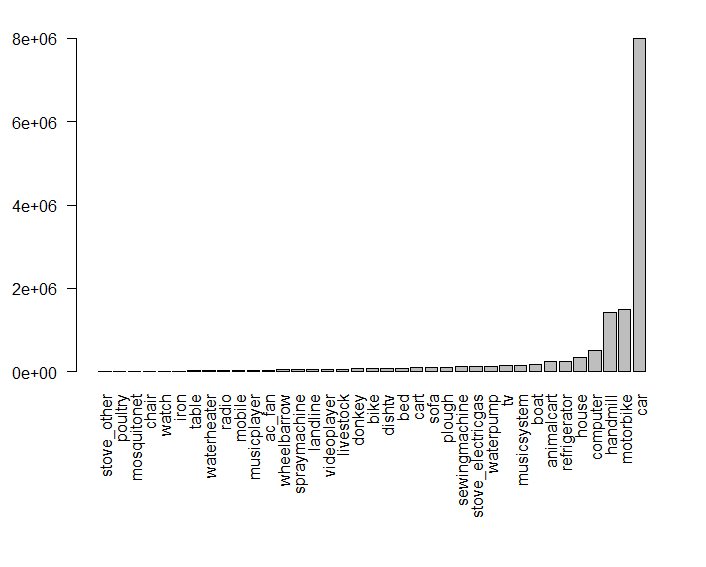
\includegraphics[width=5in,bb = 0 0 200 100, draft, type=eps]{C:/local_files/research/consumption/lsms/assets_median_cost_order2012.png}\caption{\label{fig:Costofassets2014}Cost of assets (2014)}
\end{figure}

The method to smoothen the data on the other hand has clearer advantages.
As we have noted earlier, in every two years of the survey, the mtm-average
by the household is susceptible to both how the household interviewee
may estimate the change in the market and whether the interviewee
from the household in a particular year is different from the interviewee
household member in another year. The assets data can thus be smoothened
by separating the effect of these factors if we can consider only
only one year's prices. To explain this with an example, consider
an asset $a$ whose value is $P_{a,t}\times n_{a,t}$ where $P_{a,t}$
is the reported average mtm of the asset at time $t$ and $n_{a,t}$
is the total number of assets the household possesses. To avoid the
measurement error associated with the difference in the estimate from
the year $t$ to $t+1$, we prefer to use the mtm-average estimate
(price) at either from $t$ or $t+1$. Therefore the difference in
cost of assets $a$ could be either be $P_{a,t}\times(n_{a,t+1}-n_{a,t})$
or $P_{a,t+1}\times(n_{a,t+1}-n_{a,t})$ rather than $n_{a,t+1}P_{a,t+1}-n_{a,t}P_{a,t}$.
Choosing the period $t$ however leads us to another issue due to
the sparsity of data. As we rely on a district-level granularity of
data, not only would we not have the price reported for an item not
owned by the consumer in period $t$, there may not be enough purchases
in the district for us to estimate the cost of the item that consumer
in the period $t$ (i.e. $P_{a,t}$)\footnote{One way to circumvent this is to classify all assets into cheap, middle-range
and expensive categories based on cost quantiles in the period $t$
and then determine the category of the asset purchased in $t+1$ based
on its price in $t+1$. The price at time $t$ would then by the price
of matching category (expensive, middle-range or cheap) at time $t$.
Since, we may as well use the price at $t+1$, this indirect methods
is rendered unnecessary.}. As we're interested in the price for the new purchases (i.e. cases
such that $n_{a,t}=0$ and $n_{a,t+1}>0$), the prices at $t+1$ (i.e.
$P_{a,t+1}$) do not suffer with this issue. The expenditure on new
assets calculated is thus $P_{a,t+1}$$\Delta n_{a,t+1}=P_{a,t+1}(n_{a,t+1}-n_{a,t})$
a quantity that considers an mtm change less affected by the measurement
error in the estimate provided by the household member interviewee.
In the end, we also plan to confirm the results obtained with a pseudo-panel
approach.

\begin{figure}[p]
\begin{centering}
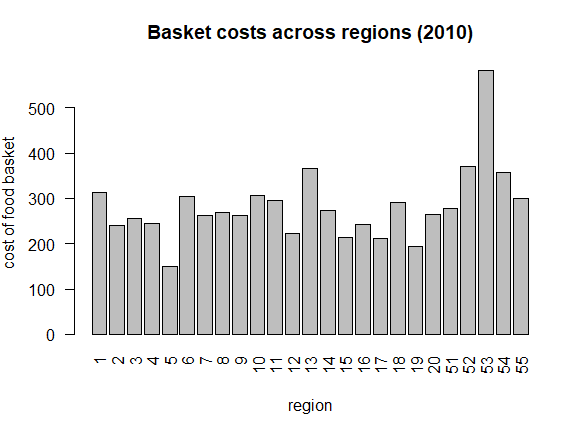
\includegraphics[width=2.5in,bb = 0 0 200 100, draft, type=eps]{C:/local_files/research/consumption/foodbasketprices_2010.png}
\par\end{centering}
\caption{\label{fig:BasketsRegions2010}The costs of the food basket across
regions in Tanzania (2010)}
\end{figure}

\begin{figure}[p]
\begin{centering}
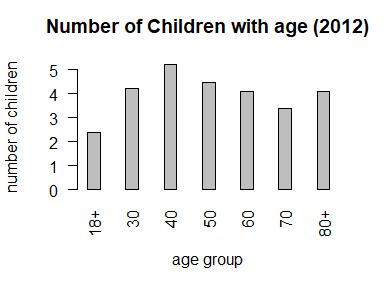
\includegraphics[width=2.5in,bb = 0 0 200 100, draft, type=eps]{C:/local_files/research/consumption/numchildren_age_2012.png}
\par\end{centering}
\caption{\label{fig:NumberChildMinYOB}Number of children living in the household
vs the age-group of the oldest member }
\end{figure}

\begin{figure}
\begin{centering}
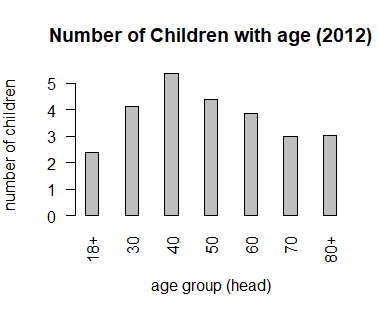
\includegraphics[width=2.5in,bb = 0 0 200 100, draft, type=eps]{C:/local_files/research/consumption/numchildren_age_head_2012.png}
\par\end{centering}
\caption{\label{fig:NumberChildhhhYOB}Number of children living in the household
vs the age-group of the (reported) household head}
\end{figure}

\begin{figure}[p]
\begin{centering}
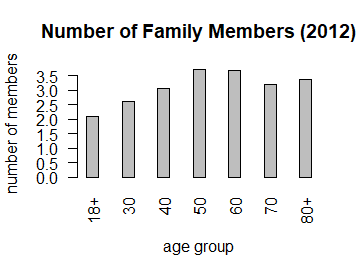
\includegraphics[width=2.5in,bb = 0 0 200 100, draft, type=eps]{C:/local_files/research/consumption/nummembers_age_occhead_2012.png}
\par\end{centering}
\caption{Number of members in the household vs the age group of the main household
earner (usually household head)}
\end{figure}


\section{\label{sec:Results}Results}

The results of the regression of $\Delta A_{\tau+1}$ against $A_{t}$
and other relevant variables are provided in the table. The results
for the regression of $\nu_{\tau+1}$ against $A_{t}$ and others
are provided in the table.

\rule[0.5ex]{1\columnwidth}{1pt}

\bibliographystyle{ieeetr}
\bibliography{C:/local_files/research/africa_attitudes}

\end{document}
